\chapter{Algorithm Performance with Common Formulas}
In this chapter we show the respective performances of the current accepted algorithm and the greedy algorithm. We do so by theoretically analyzing the general forms of four types of formulas, then computing an accepting path using both algorithms and considering and cost of the path and the time taken to calculate it.%consider the results of a practical run. %The four types of formulas we will examine are 1. Reachability while% We are able to theoretically analyze the general forms of these formulas %After we  using the FTS in figure \ref{fig:ftsEx}


%(\Pi, \rightarrow_D, \Pi_0, AP,L_D)
%This FTS will be used in figures unless otherwise stated. We chose it to be very simple because the state explosion problem applies even to the small examples in this report. If we chose a more complex FTS we would not be able to include illustrations of the product automaton because it gets very big very quickly. We will henceforth refer to this FTS as simple FTS. When providing computational results, we will use an FTS that is much larger, to bring out the difference between our algorithm and the accepted algorithm.


\section{Reachability while avoiding regions} 
Reachability while avoiding regions is a property in which we wish to not cross over certain regions, say $\pi_1, \pi_2, \dots, \pi_n$, until we get to a specified region, say $\pi_{n+1}$. After reaching $\pi_{n+1}$ we are free to do what we want. This behavior is expressed by the general formula $\neg (\pi_1 \lor \pi_2 \lor \dots \lor \pi_n) \U \pi_{n+1}$. 

\begin{figure}
\centering
\begin{tikzpicture}[->,>=stealth',shorten >=1pt,auto,node distance=2.7cm,
                    semithick]
  \tikzstyle{every state}=[fill=red,draw=black,text=black]

  \node[initial,state] (A)                    {$q_1$};
  \node[state,accepting]         (B) [right of=A] {$q_2$};

  \path (A) edge              node {$\pi_{n+1}$} (B)
  		(A) edge [loop above] node {$\neg (\pi_1 \lor \pi_2 \lor \dots \lor \pi_n)$} (A)%{$\neg \pi_1 \wedge \neg \pi_2 \wedge \dots \wedge \neg \pi_{n+1}$} (A)
  		(B) edge [loop above] node {$1$} (B);
\end{tikzpicture}
\caption{B\"{u}chi automaton corresponding to $\neg (\pi_1 \lor \pi_2 \lor \dots \lor \pi_n) \U \pi_{n+1}$}
\label{fig:ReachAvoid}
\end{figure}

The B\"{u}chi automaton corresponding to this formula is given in figure \ref{fig:ReachAvoid}. As we can see $d_p(q_1)=1$ and $d_p(q_2)=0$. In this section we will look at the specific formula $\neg \pi_4 \U \pi_5$. The product automaton of this B\"{u}chi automaton combined with the FTS from figure \ref{fig:ftsEx} is shown in figure \ref{fig:reachAvoidProduct}.

\begin{figure*}
\centering
\begin{tikzpicture}[->,>=stealth',shorten >=1pt,auto,node distance=2.3cm,
                    semithick]
  \tikzstyle{every state}=[fill=red,draw=black,text=black]

  \node[initial,state] (A)                    {\small $(\pi_1,q_1)$};
  \node[state]         (B) [ right of=A] {\small $(\pi_2,q_1)$};
  \node[state]         (C) [right of=B] {\small $(\pi_3,q_1)$};
  \node[state]         (D) [right of=C] {\small $(\pi_4,q_1)$};
  \node[state]         (E) [right of=D] {\small $(\pi_5,q_1)$};
  
  \node[state,accepting] 		   (AA)  [below of=A]  {\small $(\pi_1,q_2)$};
  \node[state,accepting]         (BB) [ right of=AA] {\small $(\pi_2,q_2)$};
  \node[state,accepting]         (CC) [right of=BB] {\small $(\pi_3,q_2)$};
  \node[state,accepting]         (DD) [right of=CC] {\small $(\pi_4,q_2)$};
  \node[state,accepting]         (EE) [right of=DD] {\small $(\pi_5,q_2)$};  

  \path (A) edge     [bend left]          (B)
        (B) edge     [bend left]          (A)
        (A) edge     [bend left]         (C)
        (C) edge     [bend left]          (A)
        %(C) edge     [bend left]          (D)
        %(D) edge     [bend left]          (C)
		%(B) edge     [bend left]          (D)
        %(D) edge     [bend left]          (B)
        (B) edge               (EE)
        (DD) edge       [bend left]        (BB)
        (BB) edge        [bend left]       (DD)
        (BB) edge        [bend left]       (AA)
        (AA) edge        [bend left]       (BB)
        (BB) edge        [bend left]       (EE)
        (EE) edge        [bend left]       (BB)
        (DD) edge       [bend left]        (CC)
        (CC) edge        [bend left]       (DD)
        (CC) edge        [bend left]       (DD)
        (DD) edge        [bend left]       (CC)
        (CC) edge        [bend left]       (AA)
        (AA) edge        [bend left]       (CC)
        (A) edge [loop above]  (A)
        (B) edge [loop above]  (B)
        (C) edge [loop above]   (C)
        %(D) edge [loop above]   (D)
        (AA) edge [loop below]  (AA)
        (BB) edge [loop below]  (BB)
        (CC) edge [loop below]  (CC)
        (DD) edge [loop below]   (DD)
        (EE) edge [loop below]   (EE);
\end{tikzpicture}
\caption{Product Automaton for $\neg \pi_4 \U \pi_5$ with Simple FTS}
\label{fig:reachAvoidProduct}
\end{figure*}
Note: in figure \ref{fig:reachAvoidProduct} all nodes have a self loop, which are not included for the sake of the reader.

To find an accepting path, the accepted algorithm starts at the initial node, $(\pi_1,q_1)$, and does a first Dijkstra search to find the optimal path to all the accepting states, $(\pi_i,q_2),$ $\forall i = 1,2,\dots,5$. Then the optimal path back from each of these accepting nodes is computed.  
 
The greedy algorithm does $n+1$ Dijkstra searches, where $n$ is the maximum level of the initial state in the B\"{u}chi automaton. As we can see in figure \ref{fig:ReachAvoid}, $n$ is 1 for all formulas of this form. Therefore, the greedy algorithm does one Dijkstra search starting from $(\pi_1,q_1)$ which ends at $(\pi_5,q_2)$. The greedy algorithm will have a slightly faster runtime because it does not find the optimal path back for every accepting node; the greedy algorithm only finds one. 

Because node $q_2$ in automaton \ref{fig:reachAvoidProduct} has a self loop and every region in the simple FTS has a self loop, every accepting state in the product automaton has a self loop. Therefore, the cost of the optimal path from any accepting node back to itself is the same, i.e.,\ 0. This implies that the accepting node that creates the optimal prefix-suffix plan, i.e.,\ $q_{f*}'$ in Procedure \ref{optrun}, is the accepting node closest to the initial node. This is the accepting node that the greedy algorithm finds, which in turn implies that both algorithms calculate the same plan. 
%%% CHECK SEMI COLON GRANT

We now investigate the computation time of both algorithms with a case study. So differences in runtime will make themselves apparent, we calculate accepting paths on a larger workspace. The workspace we will use is a grid, 25 units across and 25 units up, a total of 625 equally sized squares. Our robot can move horizontally and vertically; however, it cannot move diagonally. Additionally, the unit cost of going from any adjacent to another region is 1. The initial position is located at $(0,0)$, region $\pi_1$ is located at (2,24), region $\pi_2$ is located at (12,12), and region $\pi_3$ is located at (20,15). This workspace is seen in figure \ref{fig:workspace}.

\begin{figure}[!htb]
\centering
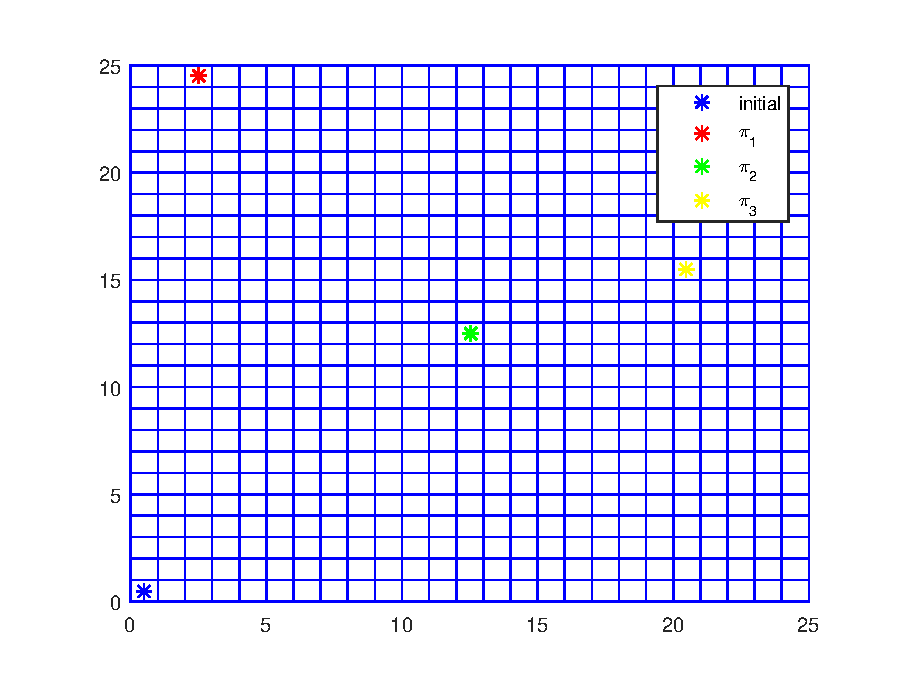
\includegraphics[scale=0.8]{workspace.eps}
\caption{Workspace 1}
\label{fig:workspace}
\end{figure}


The output from the accepted algorithm is \\


\begin{minipage}{\textwidth}
\begingroup
\fontsize{9pt}{12pt}\selectfont
\begin{lstlisting}
Accepted Algorithm
==================
accepted_plan done within 0.02s: precost 35.00, sufcost 0.00
------------------------------
the prefix of plan **states**:
[((0, 0, 1), 'None'), ((1, 0, 1), 'None'), ((2, 0, 1), 'None'), ((3, 0, 1), 'None'), ((3, 1, 1), 'None'), ((4, 1, 1), 'None'), ((5, 1, 1), 'None'), ((6, 1, 1), 'None'), ((6, 2, 1), 'None'), ((6, 3, 1), 'None'), ((6, 4, 1), 'None'), ((6, 5, 1), 'None'), ((7, 5, 1), 'None'), ((8, 5, 1), 'None'), ((8, 6, 1), 'None'), ((9, 6, 1), 'None'), ((10, 6, 1), 'None'), ((10, 7, 1), 'None'), ((10, 8, 1), 'None'), ((10, 9, 1), 'None'), ((11, 9, 1), 'None'), ((12, 9, 1), 'None'), ((12, 10, 1), 'None'), ((13, 10, 1), 'None'), ((14, 10, 1), 'None'), ((14, 11, 1), 'None'), ((15, 11, 1), 'None'), ((16, 11, 1), 'None'), ((17, 11, 1), 'None'), ((18, 11, 1), 'None'), ((19, 11, 1), 'None'), ((19, 12, 1), 'None'), ((20, 12, 1), 'None'), ((20, 13, 1), 'None'), ((20, 14, 1), 'None'), ((20, 15, 1), 'None'), ((20, 15, 1), 'None')]
the suffix of plan **states**:
[((20, 15, 1), 'None'), ((20, 15, 1), 'None')]
------------------------------
the prefix of plan **actions**:
[(0, 0, 1), (1, 0, 1), (2, 0, 1), (3, 0, 1), (3, 1, 1), (4, 1, 1), (5, 1, 1), (6, 1, 1), (6, 2, 1), (6, 3, 1), (6, 4, 1), (6, 5, 1), (7, 5, 1), (8, 5, 1), (8, 6, 1), (9, 6, 1), (10, 6, 1), (10, 7, 1), (10, 8, 1), (10, 9, 1), (11, 9, 1), (12, 9, 1), (12, 10, 1), (13, 10, 1), (14, 10, 1), (14, 11, 1), (15, 11, 1), (16, 11, 1), (17, 11, 1), (18, 11, 1), (19, 11, 1), (19, 12, 1), (20, 12, 1), (20, 13, 1), (20, 14, 1), (20, 15, 1), 'None', 'None']
the suffix of plan **actions**:
['None', 'None']
full construction and synthesis done within 0.11s
\end{lstlisting}
\endgroup
\end{minipage} \\ \\


The output of the algorithm is structured as follows: the time taken to calculate the path, the cost of the prefix, and the cost of the suffix are given at the top of the output. The following sequence of \texttt{states} can be thought of as the result of the labelling function in Definition \ref{defDLF}, and \texttt{actions} can be thought of as the labels of the transition of the B\"uchi automaton. The \texttt{full construction and synthesis} includes the time taken to construct the graph, thus it is larger than the first time given. The construction of the graph almost always takes the majority of time. For the rest of this report, the calculated paths will appear in the appendix.% for the ease of the reader.

The greedy algorithm outputs the same plan marginally faster. \\


\begin{minipage}{\textwidth}
\begingroup
\fontsize{9pt}{12pt}\selectfont
\begin{lstlisting}
Greedy Algorithm
================
greedy_plan done within 0.01s: precost 35.00, sufcost 0.00
...
full construction and synthesis done within 0.10s 
\end{lstlisting}
\endgroup
\end{minipage} \\ \\


%As we can see, our algorithm computed the same path in about the same time.%seconds. This may seem weird because we have shown that our algorithm does the same calculation when finding a path from the initial node to an accepting node. The difference is that for each accepting node, a Dijkstra search is performed. In this example, there are 625 accepting states (the number of states in the FTS times the number of states in the B\"uchi automaton). The function \texttt{dijkstra\_predecessor\_and\_distance} from \cite{schult08} is used to calculate the shortest path back to an accepting node. 
\section{Sequencing}
Sequencing is the behavior of visiting regions $\pi_1,\pi_2,\dots,\pi_n$ in that order. One example of a formula of this type is $\diamond (\pi_3 \land  \diamond \pi_5)$, and the corresponding B\"uchi automaton is shown in figure \ref{fig:seq}. We note that this automaton is only applicable because of the partition we defined earlier in Definition \ref{def:PM}, which makes it impossible for $\pi_i$ and $\pi_j$ to be true at the same time if $i\neq j$. The LTL2BA tool \cite{ltlbuchiwebsite} that is used generates an automaton with an edge from $q_1$ to $q_3$ labelled $\pi_3 \&\& \pi_5 $. This transition is impossible so we take it out before calculating the distances. The greedy algorithm would not work if every state in the B\"uchi automaton had a distance of 1 and the accepting states had a distance of 0. The product automaton of formula $\diamond (\pi_3 \wedge \diamond \pi_5)$, the simple FTS, is shown in figure \ref{fig:Sequencing}.


\begin{figure}
\centering
\begin{tikzpicture}[->,>=stealth',shorten >=1pt,auto,node distance=2.8cm,
                    semithick]
  \tikzstyle{every state}=[fill=red,draw=black,text=black]

  \node[initial,state] (A)                    {$q_1$};
  %\node[state] (B)                    [right of=A]{$q_2$};
  \node[state] (B)                    [right of=A]{$q_2$};
  \node[state,accepting]         (C) [right of=B] {$q_3$};

  \path (A) edge              node {$\pi_{3}$} (B)
  		(A) edge [loop above] node {$\neg \pi_3$} (A)
  		(B) edge [loop above] node {$\neg \pi_5$} (B)
  		(B) edge              node {$\pi_{5}$} (C)
  		(C) edge [loop above] node {$1$} (C);
%  		(C) edge              node {$\pi_{3}$} (D)
 % 		(D) edge [loop above] node {$1$} (D);
\end{tikzpicture}
\caption{B\"uchi Automaton Corresponding to $  \diamond(\pi_3 \land \diamond \pi_5)$}
\label{fig:seq}
\end{figure}

\begin{figure*}
\centering
\begin{tikzpicture}[->,>=stealth',shorten >=1pt,auto,node distance=2.6cm,
                    semithick]
  \tikzstyle{every state}=[fill=red,draw=black,text=black]

  \node[initial,state] (A)                    {\footnotesize $(\pi_1,q_1)$};
  \node[state]         (B) [ right of=A] {\footnotesize $(\pi_2,q_1)$};
  \node[state]         (C) [right of=B] {\footnotesize $(\pi_3,q_1)$};
  \node[state]         (D) [right of=C] {\footnotesize $(\pi_4,q_1)$};
  \node[state]         (E) [right of=D] {\footnotesize $(\pi_5,q_1)$};
  
  \node[state] 		   (AA)  [below of=A]  {\footnotesize $(\pi_1,q_2)$};
  \node[state]         (BB) [ right of=AA] {\footnotesize $(\pi_2,q_2)$};
  \node[state]         (CC) [right of=BB] {\footnotesize $(\pi_3,q_2)$};
  \node[state]         (DD) [right of=CC] {\footnotesize $(\pi_4,q_2)$};
  \node[state]         (EE) [right of=DD] {\footnotesize $(\pi_5,q_2)$};
  
  \node[state,accepting] 		   (AAA)  [below of=AA]  {\footnotesize $(\pi_1,q_3)$};
  \node[state,accepting]         (BBB) [ right of=AAA] {\footnotesize $(\pi_2,q_3)$};
  \node[state,accepting]         (CCC) [right of=BBB] {\footnotesize $(\pi_3,q_3)$};
  \node[state,accepting]         (DDD) [right of=CCC] {\footnotesize $(\pi_4,q_3)$};
  \node[state,accepting]         (EEE) [right of=DDD] {\footnotesize $(\pi_5,q_3)$};
  

  \path (A) edge     [bend left]          (B)
        (B) edge     [bend left]          (A)
        %(A) edge     [bend left]         (C)
        %(C) edge     [bend left]          (A)
        %(C) edge		[bend left] 		(D)
        %(D) edge 		[bend left]      (C)
        (A) edge               (CC)
        %(BB) edge               (EEE)
        (BB)	edge			[loop above] (BB)
        (AA)	edge			[loop above] (AA)
        (CC)	edge			[loop above] (CC)
        (DD)	edge			[loop above] (DD)
        (A)	edge			[loop above] (A)
        (E)	edge			[loop above] (E)
        (D)	edge			[loop above] (D)
        (AAA)	edge			[loop below] (AAA)
        (BBB)	edge			[loop below] (BBB)
        (CCC)	edge			[loop below] (CCC)
        (DDD)	edge			[loop below] (DDD)
        (EEE)	edge			[loop below] (EEE)
        (D) edge               (CC)
        (B) edge       [bend left]        (E)
        (E) edge       [bend left]        (B)
        (B) edge       [bend left]        (D)
        (D) edge       [bend left]        (B)
        (BB) edge 			(EEE)
%        (EE) edge			[bend left]		(BB)
        (DD) edge       [bend left]        (BB)
        (BB) edge        [bend left]       (DD)
        (BB) edge        [bend left]       (AA)
        (AA) edge        [bend left]       (BB)
        (CC) edge        [bend left]       (AA)
        (AA) edge        [bend left]       (CC)
        (CC) edge        [bend left]       (DD)
        (DD) edge        [bend left]       (CC)
        
        (DDD) edge       [bend left]        (BBB)
        (BBB) edge        [bend left]       (DDD)
        (BBB) edge        [bend left]       (AAA)
        (AAA) edge        [bend left]       (BBB)
        (BBB) edge        [bend left]       (EEE)
        (EEE) edge        [bend left]       (BBB)
        (DDD) edge       [bend left]        (CCC)
        (CCC) edge        [bend left]       (DDD)
        (CCC) edge        [bend left]       (DDD)
        (DDD) edge        [bend left]       (CCC)
        (CCC) edge        [bend left]       (AAA)
        (AAA) edge        [bend left]       (CCC);
\end{tikzpicture}
\caption{Product Automaton for $\diamond (\pi_4 \wedge \diamond \pi_5)$ with Simple FTS}
\label{fig:Sequencing}
\end{figure*}

We look at how the two algorithms will search this product automaton to find an accepting path. The accepted algorithm starts at the initial node $(\pi_1,q_1)$ and in the first step searches the nodes connected to $(\pi_1,q_1)$, i.e.,\ $(\pi_2,q_1)$ and $(\pi_3,q_2)$. In the next step it searches $(\pi_4,q_1)$, $(\pi_5,q_1)$, $(\pi_1,q_2)$, $(\pi_4,q_2)$. Next it searches $(\pi_2,q_2)$ and then $(\pi_5,q_3)$. Even though $(\pi_5,q_3)$ is an accepting state, the accepted algorithm continues the search because it has to find the shortest path to \textit{all} accepting nodes. In the next step it searches $(\pi_2,q_3)$, then $(\pi_1,q_3)$ and $(\pi_4,q_3)$ and finally $(\pi_3,q_3)$. After this, it finds the shortest path from all accepting nodes back to themselves. Again, every accepting node has a self loop so all the accepting nodes have a suffix cost of 0. 



The greedy algorithm also starts at $(\pi_1,q_1)$ and in the first step searches $(\pi_2,q_1)$ and $(\pi_3,q_2)$. The greedy algorithm notices that the current level is 2, and $(\pi_3,q_2)$ is on level 1. Because the level of $(\pi_3,q_2)$ is 1 below the current level, the greedy algorithm finishes the Dijkstra search and starts another Dijkstra search beginning at $(\pi_3,q_2)$. In the first step, $(\pi_1,q_2)$ and $(\pi_4,q_2)$ are searched. It will then do another step and search $(\pi_2,q_2)$. Finally in the third step, it searches $(\pi_5,q_3)$. It notices $(\pi_5,q_3)$ is an accepting state and finishes the search. It then finds the optimal path from $(\pi_5,q_3)$ back to itself.

We run both algorithms with the formula $\diamond (\pi_1 \land \diamond(\pi_2 \land \diamond \pi_3))$ and Workspace 1 in figure \ref{fig:workspace}. The output of the accepted algorithm is \\


\begin{minipage}{\textwidth}
\begingroup
\fontsize{9pt}{12pt}\selectfont
\begin{lstlisting}
Accepted Algorithm
==================
accepted_plan done within 0.04s: precost 62.00, sufcost 0.00
...
full construction and synthesis done within 0.19s 
\end{lstlisting}
\endgroup
\end{minipage} \\ \\


The greedy algorithm computed the same path with an output of \\


\begin{minipage}{\textwidth}
\begingroup
\fontsize{9pt}{12pt}\selectfont
\begin{lstlisting}
Greedy Algorithm
================
greedy_plan done within 0.02s: precost 62.00, sufcost 0.00
...
full construction and synthesis done within 0.17s 
\end{lstlisting}
\endgroup
\end{minipage} \\ \\


As we can see, the plan synthesis took the greedy algorithm half as long; 0.02 seconds compared to 0.04 seconds. We take a look at what causes the increased time. 

\begin{figure}[!htb]
\centering
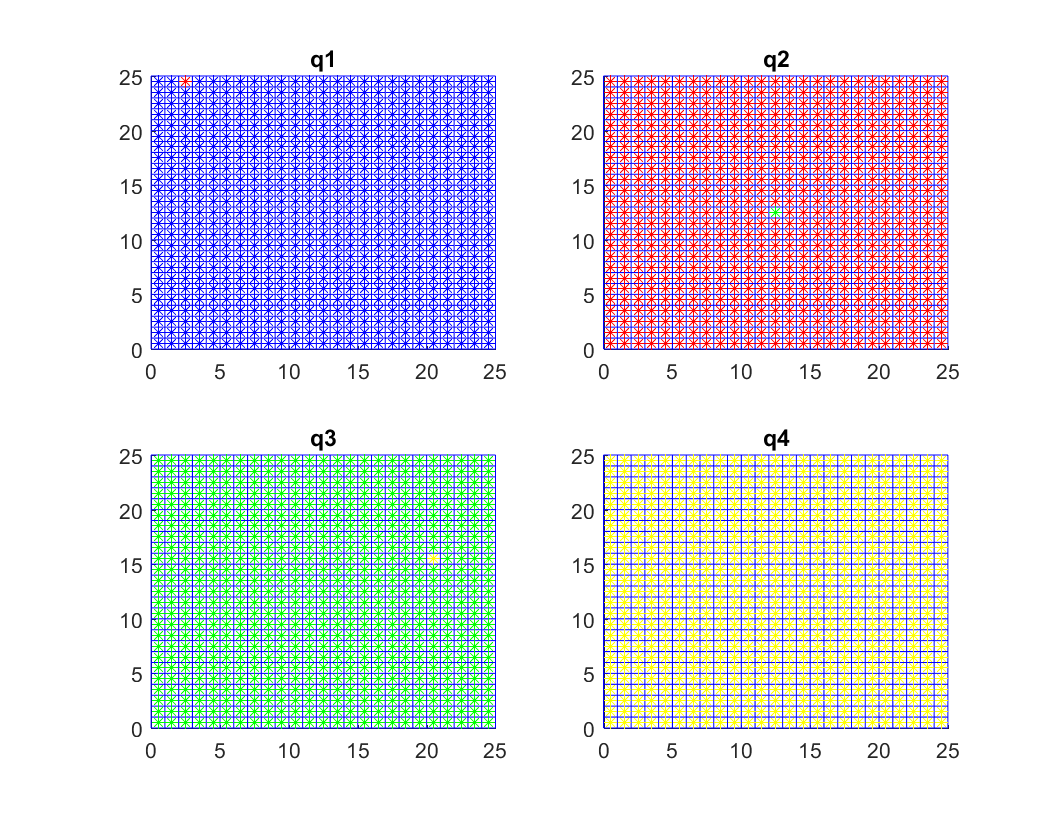
\includegraphics[scale=0.7]{acceptedPlot}
\caption{Nodes searched with the accepted algorithm}
\label{fig:animAccept}
\end{figure}

\begin{figure}[!htb]
\centering
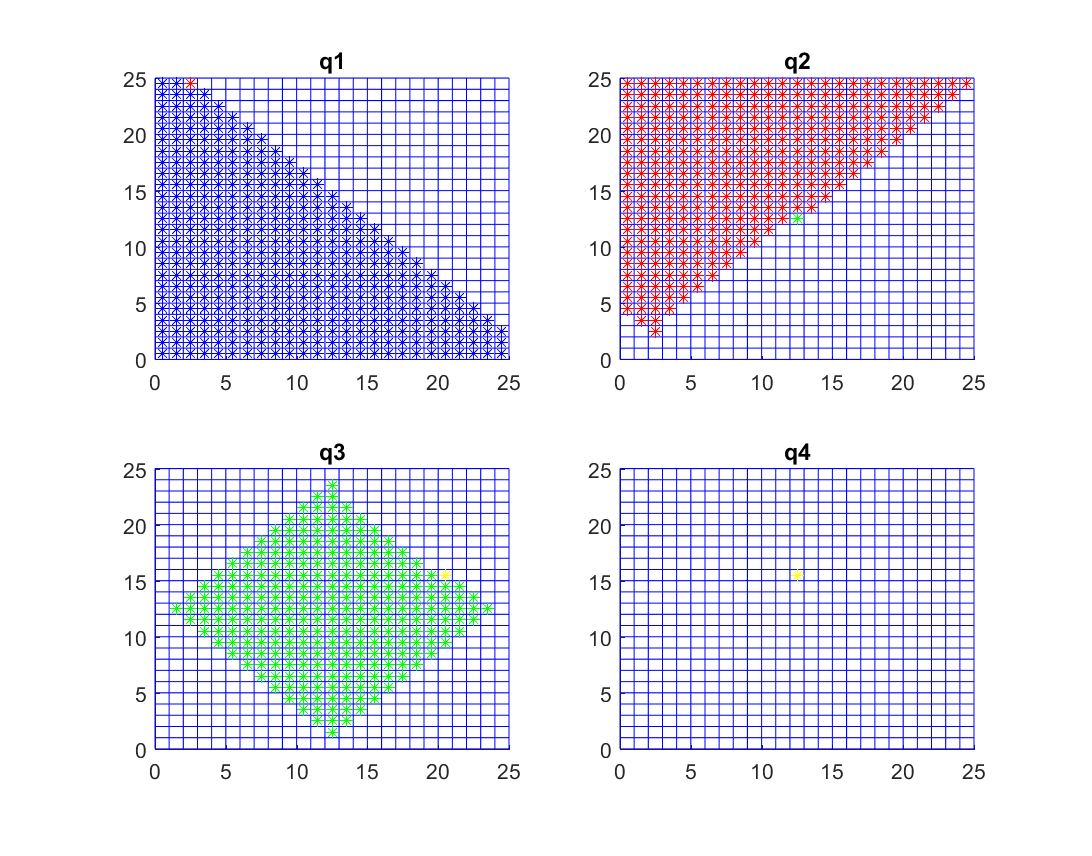
\includegraphics[scale=0.7]{ourPlot}
\caption{Nodes searched with the greedy algorithm}
\label{fig:animOur}
\end{figure}

Figure \ref{fig:animAccept} shows the states searched with the accepted algorithm and figure \ref{fig:animOur} shows the states searched with the greedy algorithm. Each figure shows a representation of the product automaton. The graph can be thought of as the discretization of the workspace, and there are four corresponding to the four states in the B\"uchi automaton. Any square filled in with blue, red, green, or yellow has been visited, all others have not. As we can see, the greedy algorithm searches a significantly smaller number of nodes, while the accepted algorithm searches every node.

The FTS has 625 states and the B\"uchi automaton has four states, which implies the product automaton has 2500 states. The accepted algorithm does one Dijkstra search from the initial node to each of the 2499 other nodes, and then computes the suffix cost for each of the 625 accepting nodes. The algorithm then chooses which combination out of the 625 choices makes the shortest overall run. 

The level of the initial node is three, so the greedy algorithm does three Dijkstra searches: one for each level and one for the accepted node back to itself. To find an accepting node, the first search searches through 326 nodes, the second 266 nodes, and the third 587 nodes. The last search simply finds the path from the accepting node back to itself, which is a self loop. Thus the greedy algorithm searches 1179 nodes compared to 2500 nodes.  
%Check how many nodes are searched with both algorithms, and show time difference.

Because there is only one way down at each level, the concatenation of the locally optimal paths will be the globally optimal path. Then the advantage that the greedy algorithm has over the accepted algorithm is that the accepted algorithm will search through more extraneous nodes. Because all accepting nodes have the same suffix cost, the optimal accepting node will be the one closest to the initial node. This is the one the greedy algorithm finds. Thus the greedy algorithm is guaranteed to find the optimal path in a shorter amount of time than the accepted algorithm.


\section{Coverage}
A coverage formula represents the statement, visit $\pi_1, \pi_2, \dots, \pi_n$ in any order, and is of the form $\varphi = \diamond \pi_1 \wedge \diamond \pi_2 \wedge \dots \wedge \diamond \pi_n$. We show the B\"uchi automaton corresponding to the formula $\diamond \pi_1 \wedge \diamond \pi_2 \wedge \diamond \pi_3$ in figure \ref{fig:buchCov}.

\begin{figure}
\centering
\begin{tikzpicture}[->,>=stealth',shorten >=1pt,auto,node distance=3.3cm,
                    semithick]
  \tikzstyle{every state}=[fill=red,draw=black,text=black]

  \node[initial,state] (A)                    {\small $q_1$};
  \node[state] (C)                    [below of=A]{\small $q_3$};
  \node[state] (D)                    [right of=C]{\small $q_4$};
  \node[state]         (B) [left of=C] {\small $q_2$};
  \node[state] (E) 					[below of=B]{\small $q_5$};
   \node[state] (F) 					[below of=C]{\small $q_6$};
   \node[state] (G) 					[below of=D]{\small $q_7$};
   \node[accepting,state] (H) 					[below of=F]{\small $q_8$};
  

  \path (A) edge              node {\small $\pi_{1}$} (B)
   (A) edge              node {\small $\pi_{2}$} (C)
   (A) edge              node {\small $\pi_{3}$} (D)
   (B) edge              node {\small $\pi_{2}$} (E)
   (B) edge              node [near start] {\small $\pi_{3}$} (F)
   (C) edge              node [near end] {\small $\pi_{1}$} (E)
   (E) edge              node {\small $\pi_{3}$} (H)
   (F) edge              node {\small $\pi_{2}$} (H)
   (G) edge              node {\small $\pi_{1}$} (H)
   (D) edge              node {\small $\pi_{2}$} (G)
   (A) edge      [loop above]        node {\small $\neg (\pi_1 \lor \pi_{2} \lor\pi_3)$} (A)
   (B) edge      [loop left]        node {\small $\neg (\pi_{2} \lor \pi_3)$} (B)
   (C) edge      [loop below]        node {\small $\neg( \pi_1 \lor \pi_3)$} (C)
   (D) edge      [loop right]        node {\small $\neg (\pi_1 \lor \pi_{2}) $} (A)
   (E) edge      [loop left]        node {\small $\neg  \pi_3$} (E)
   (F) edge      [loop above]        node {\small $\neg  \pi_2$} (F)
   (G) edge      [loop right]        node {\small $\neg  \pi_1$} (G)
   (H) edge      [loop below]        node {\small $1$} (H)
   (D) edge              node [near start] {\small $\pi_{1}$} (F)
   (C) edge              node [near start] {\small $\pi_{3}$} (G);
\end{tikzpicture}
\caption{B\"uchi Automaton Corresponding to $\diamond \pi_1 \wedge \diamond \pi_2 \wedge \diamond \pi_3$}
\label{fig:buchCov}
\end{figure}

We can see that to get to the accepting node, we have to choose which node to go to first, and then which node to go to second (the third node we then have to visit is already decided). So, there are 6 possible paths to take from the initial node, $q_1$ to accepting state $q_8$. This is true in the product automaton too, if we only consider the option of taking the optimal path between nodes. 

The accepted algorithm will search through the whole product automaton and will then choose the order that produces the global minimum. The greedy algorithm, on the other hand, will first choose $\pi_i$, which is the closest to the initial node. From there, it will choose $\pi_j$, which is closest to $\pi_i$ out of the two that have not been visited yet. Thus the greedy algorithm may not compute the globally optimal path on a coverage formula. It will, however, compute an accepting path with a bound on the cost of the greedy path in terms of the cost of the optimal path. 

To prove this cost bound, we first show that this path corresponds to the one generated by the nearest neighbor approach to the travelling salesperson problem. Next we provide the bound on the cost of our path based on the worst case ratio of the nearest neighbor path to the optimal path given by Rosendrantz, Stearns, and Lewis \cite{rosenkrantz74}. 

%This problem is NP-hard, 
\subsection{Travelling Salesperson Problem}
The travelling salesperson problem is stated in layman's terms as finding the shortest path for a salesperson to take such that he passes through a given set of cities and then returns back home at the end. This problem has been studied extensively, and many algorithms and heuristics exist for finding an approximate solution. One very simple algorithm to do this is called the nearest neighbor algorithm. It says from the starting city, pick the closest city to be the next stop. From there, pick the next closest city not including the starting city, and so on. If there is a tie in the next closest neighbor, the next node can be decided arbitrarily. This is exactly what the greedy algorithm does when given a coverage formula; the first Dijkstra search finds the closest node, we start another search from that node, and so on. 

To formulate our problem as a travelling salesperson problem we use the idea of a dummy node from the computer wiring example in \cite{lenstra75}. In the example, a computer interface is being designed at the Institute for Nuclear Physical Research in Amsterdam. An interface is made up of several modules, with multiple pins on each module. A given subset of pins has to be interconnnected by wires, and at most two wires can be connected to any pin. For obvious reasons, it is desirable to minimize the amount of wire used. They show that this problem can be formulated as a travelling salesperson problem. The only difference between this problem and a travelling salesperson problem is that in the travelling salesperson problem, the salesperson must return home at the end. This is not true in this problem. It is also not true in our problem, we only need to pass through $\pi_1$, $\pi_2$ and $\pi_3$ and there is no need to return to the starting state after we do this. To formulate this problem as a travelling salesperson problem, they set $P$ to be the set of pins to be interconnected, and $c_{ij}$ to be the distance between pin $i$ and pin $j$. They then introduce a dummy node $*$ that is a distance 0 from all the other nodes, i.e.,\ $c_{i*} = c_{*i} = 0$ for all i. Then the corresponding problem is solving the travelling salesperson problem on the set of nodes $N=P \cup \{*\}$. 

For our problem, we set $c_{ij}=d(\pi_i , \pi_j)$ for $i,j=0,1,2,3$, where the initial state is from now on known as $\pi_0$, to be the shortest path our robot can take from $\pi_i$ to $\pi_j$. When introducing the dummy node, we must preserve the the triangle inequality for a proof of a worst case scenario bound we will provide later on. To do this, we cannot have the dummy node be distance 0 from the other nodes. Indeed, if $c_{i*} = c_{*i} = 0 $ the triangle inequality would be violated because $c_{i*} + c_{*j} = 0 \leq c_{ij}$.

We can represent the relationship between the regions in our graph with the following \textit{complete} subgraph, shown in figure \ref{fig:completeGraph}. A complete graph is an undirected graph in which every pair of vertices is connected by an edge. 
\begin{figure}
\centering
\begin{tikzpicture}[-,>=stealth',shorten >=1pt,auto,node distance=5cm,
                    semithick]
  \tikzstyle{every state}=[fill=red,draw=black,text=black]

  \node[state] (A)                    {$\pi_0$};
  \node[state] (B)                    [right of=A]{$\pi_1$};
  \node[state] (C)                    [below of=A]{$\pi_2$};
  \node[state]         (D) [right of=C] {$\pi_3$};

  \path (A) edge              node {$26$} (B)
  		(A) edge 			 node {$24$} (C)
  		(A) edge              node [near start] {$35$} (D)
  		(B) edge 				node [near start] {$22$} (C)
  		(B) edge              node {$27$} (D)
  		(C) edge				node {$11$} (D);
\end{tikzpicture}
\caption{Complete Graph between Regions of Interest}
\label{fig:completeGraph}
\end{figure}

For the distances, we use the so called \textit{Manhattan distance}, i.e.,\ \\ $d((x_1,y_1),(x_2,y_2)) = |x_1 - x_2| +| y_1 - y_2|$ because our robot can only move horizontally and vertically, not diagonally. Given the weights between the vertices, we easily see that the path that the greedy algorithm will take is shown in figure \ref{fig:pathOnComplete}. The cost of this path is 62. However, this is not the optimal path, which is shown in figure \ref{fig:optcompleteGraph} and has a cost of 59.

\begin{figure}
\centering
\begin{tikzpicture}[-,>=stealth',shorten >=1pt,auto,node distance=4cm,
                    semithick]
  \tikzstyle{every state}=[fill=red,draw=black,text=black]

  \node[state] (A)                    {$\pi_0$};
  \node[state] (B)                    [right of=A]{$\pi_1$};
  \node[state] (C)                    [below of=A]{$\pi_2$};
  \node[state]         (D) [right of=C] {$\pi_3$};

  \path (A) edge 			 node {$24$} (C)
  		(B) edge              node {$27$} (D)
  		(C) edge				node {$11$} (D);
\end{tikzpicture}
\caption{Nearest Neighbor Path}
\label{fig:pathOnComplete}
\end{figure}


\begin{figure}
\centering
\begin{tikzpicture}[-,>=stealth',shorten >=1pt,auto,node distance=4cm,
                    semithick]
  \tikzstyle{every state}=[fill=red,draw=black,text=black]

  \node[state] (A)                    {$\pi_0$};
  \node[state] (B)                    [right of=A]{$\pi_1$};
  \node[state] (C)                    [below of=A]{$\pi_2$};
  \node[state]         (D) [right of=C] {$\pi_3$};

  \path (A) edge              node {$26$} (B)
  		%(A) edge 			 node {$24$} (C)
  		%(A) edge              node {$35$} (D)
  		(B) edge 				node {$22$} (C)
  		%(B) edge              node {$27$} (D)
  		(C) edge				node {$11$} (D);
\end{tikzpicture}
\caption{Optimal Path}
\label{fig:optcompleteGraph}
\end{figure}


Because we have to make sure that the dummy node does not change the order that the greedy algorithm and the nearest neighbor algorithm take we have to set the distance of the dummy node from every other node to be $\max_{i,j} c_{ij} $ where $c_{ij}$ is the distance between the nodes in the complete subgraph in figure \ref{fig:completeGraph}. In our case, this is 35, the path between $\pi_0$ and $\pi_3$. This insures that the path taken by the greedy algorithm is the same as the nearest neighbor algorithm because the dummy node will be the last node to be visited. Thus, the only time when it is a possibility that the nearest neighbor algorithm goes to the dummy node, i.e.,\ when the next node is $\max_{i,j} c_{ij}$ from the current node, is when and if we are faced with the only choice being to take the maximum path $ \max_{i,j} \hspace{0.1cm} c_{i,j}$ to $\pi_j$ or to go to the dummy node. We say we go to $\pi_j$ because the ties can be broken arbitrarily. In any other case, the nearest neighbor path will choose to go to a node where the cost is $c_{i',j'} < c_{i,j}$. We show the new subgraph in figure \ref{fig:completeDummy}

\begin{figure}
\centering
\begin{tikzpicture}[-,>=stealth',shorten >=1pt,auto,node distance=5cm,
                    semithick]
  \tikzstyle{every state}=[fill=red,draw=black,text=black]

  \node[state] (A)                    {$\pi_0$};
  \node[state] (B)                    [right of=A]{$\pi_1$};
  \node[state] (C)                    [below of=A]{$\pi_2$};
  \node[state]         (D) [right of=C] {$\pi_3$};
  \node[state] (E)			[right of = D] {$*$}; 

  \path (A) edge              node {$26$} (B)
  		(A) edge 			 node {$24$} (C)
  		(A) edge              node [near end] {$35$} (D)
  		(B) edge 				node [near end] {$22$} (C)
  		(B) edge              node [near start] {$27$} (D)
  		(C) edge				node {$11$} (D)
  		(E) edge 				node {$35$} (D)
  		(E) edge 				[bend left] node {$35$} (C)
  		(E) edge 				node {$35$} (B)
  		(E) edge 				node [near start] {$35$} (A);
\end{tikzpicture}
\caption{Complete Subgraph with Dummy Node}
\label{fig:completeDummy}
\end{figure}

The path that the nearest neighbor algorithm takes in this situation is given in figure \ref{fig:NearNeigDummy}, which gives a total cost of 132. Again, this is not the optimal solution. The optimal solution is shown in figure \ref{fig:optDummy} and has a cost of 129.

\begin{figure}
\centering
\begin{tikzpicture}[-,>=stealth',shorten >=1pt,auto,node distance=4cm,
                    semithick]
  \tikzstyle{every state}=[fill=red,draw=black,text=black]

  \node[state] (A)                    {$\pi_0$};
  \node[state] (B)                    [right of=A]{$\pi_1$};
  \node[state] (C)                    [below of=A]{$\pi_2$};
  \node[state]         (D) [right of=C] {$\pi_3$};
  \node[state] (E)			[right of = D] {$*$}; 

  \path (A) edge 			 node {$24$} (C)
  		%(A) edge              node {$35$} (D)
  		%(B) edge 				node {$22$} (C)
  		(B) edge              node [near start] {$27$} (D)
  		(C) edge				node {$11$} (D)
  		%(E) edge 				node {$35$} (D)
  		%(E) edge 				[bend left] node {$35$} (C)
  		(E) edge 				node {$35$} (B)
  		(E) edge 				node [near start] {$35$} (A);
\end{tikzpicture}
\caption{Nearest Neighbor Path with Dummy Node}
\label{fig:NearNeigDummy}
\end{figure}


\begin{figure}
\centering
\begin{tikzpicture}[-,>=stealth',shorten >=1pt,auto,node distance=4cm,
                    semithick]
  \tikzstyle{every state}=[fill=red,draw=black,text=black]

  \node[state] (A)                    {$\pi_0$};
  \node[state] (B)                    [right of=A]{$\pi_1$};
  \node[state] (C)                    [below of=A]{$\pi_2$};
  \node[state]         (D) [right of=C] {$\pi_3$};
  \node[state] (E)			[right of = D] {$*$}; 

  \path (A) edge			node {$26$} (B)
  		%(A) edge 			 node {$24$} (C)
  		%(A) edge              node {$35$} (D)
  		(B) edge 				node {$22$} (C)
  		%(B) edge              node {$27$} (D)
  		(C) edge				node {$11$} (D)
  		(E) edge 				node {$35$} (D)
  		%(E) edge 				[bend left] node {$35$} (C)
  		%(E) edge 				node {$35$} (B)
  		(E) edge 				node {$35$} (A);
\end{tikzpicture}
\caption{Optimal Path with Dummy Node}
\label{fig:optDummy}
\end{figure}


\subsection{Cost Bound}

It has been shown \cite{rosenkrantz74} that for an n-node travelling salesperson problem which satisfies the triangle inequality, i.e.,\ $d(i,j) + d(j,k) \geq d(i,k)$ for all $i,j,$ and $k$ where $d(i,j)$ is the nonnegative distance between nodes $i$ and $j$, 
\begin{align*}
\text{NEARNEIBR} \leq (\frac{1}{2} \lceil \log(n) \rceil + \frac{1}{2})\text{OPTIMAL}
\end{align*}
where NEARNEIBR is the cost of the path generated by the nearest neighbor algorithm and OPTIMAL is the cost of the optimal path. 

Our values do indeed satisfy this inequality
\begin{align*}
\text{NEARNEIBR} &\leq (\frac{1}{2} \lceil \log(n) \rceil + \frac{1}{2})\text{OPTIMAL} \\
132 &\leq (\frac{1}{2} \lceil \log(5) \rceil + \frac{1}{2})129 \\
132 &\leq 258 
\end{align*}
We also see that it is a very conservative worst case bound and we will likely do much better.

We provide a proof of
\begin{align}
\dfrac{\text{NEARNEIBR}}{\text{OPTIMAL}} \leq \frac{1}{2} \lceil \log(n) \rceil + \frac{1}{2}
\end{align}
which can be found in \cite{rosenkrantz74}. 
Proof:
We begin by proving 
\begin{align}
\text{OPTIMAL} \geq 2 \sum^{\min(2k,n)}_{i=k+1} l_i \label{eq:showFirst}
\end{align}
for all $k$, $0\leq k \leq n$. 
Let $l_i$ be the length of the $i^{th}$ largest edge in the path obtained by the nearest neighbor algorithm. For each $i$, $0 \leq i \leq n$, let $a_i$ be the node \textit{onto which} the $i^{th}$ largest edge is added (that would be the edge with length $l_i$). Let $H$ be the complete subgraph defined on the set of nodes $\{a_i \hspace{0.1cm} | \hspace{0.1cm} 1 \leq i \leq min(2k,n)\}$.

Now, let $T$ be the path in $H$ which visits the nodes of $H$ in the same order as these nodes are visited in an optimal path of the original graph. Let LENGTH be the length of $T$. We have 
\begin{align}
\text{OPTIMAL $\geq$ LENGTH} \label{eq:optglen}
\end{align}
This is because the path with cost OPTIMAL passes through all the nodes that the path with cost LENGTH passes through, and more. Thus, if H has an edge $(b,c)$, then the OPTIMAL path will either have the edge $(b,c)$ or take a less direct route through some of its extra nodes. So the triangle inequality implies (\ref{eq:optglen}).  
   
Let $(a_i,a_j)$ be an edge of $T$. If the nearest neighbor method adds point $a_i$ before $a_j$, we have $d(a_i,a_j) \geq l_i$, where $d(a_i,a_j)$ is the distance between nodes $a_i$ and $a_j$. We also see that if $a_j$ is added first, we have $d(a_i, a_j) \geq l_j$. This is because, say we added $a_i$ first, we know there is a point $l_i$ away from $a_i$ that the nearest neighbor method makes the path to. This can be $a_j$ because we know $a_j$ has not been added yet. It can also be another node, and if it is another node $d(a_i, a_j) \geq l_i$ because the nearest neighbor finds the closest node that has not yet been visited. On the other hand, if $a_j$ is added next, $d(a_i, a_j) = l_i$. 

Since one has to be added before the other, we have 
\begin{align}
d(a_i , a_j) \geq \min(l_i, l_j) \label{ex:oneBefore}
\end{align}

Summing (\ref{ex:oneBefore}) over the edges of $T$, we get
\begin{align}
\text{LENGTH} \geq \sum_{(a_i,a_j) \text{ in } T} \min(l_i,l_j)  \label{eq:lengmin}
\end{align}

If we let $\alpha_i$ be the number of edges $(a_i, a_j)$ in $T$ for which $l_i$ is selected as $\min(l_i, l_j)$ we obtain 

\begin{align}
\sum_{(a_i,a_j) \text{ in } T} \min(l_i, l_j) = \sum_{a_i \text{ in } H} \beta_i l_i  \label{ex:lowBound}
\end{align}

Because $a_i$ is the endpoint of two edges in $T$, $\beta_i \leq 2$ $\forall i$. Because $T$ has $\min(2k,n)$ edges (one for each node),

\begin{align}
\sum_{a_i \text{ in } H} \beta_i = \min(2k,n) 
\end{align}

To get a lower bound on (\ref{ex:lowBound}), we assume that $\beta_i = 2 $ for $k+1 \leq i \leq \min(2k,n)$ and is zero of $i \leq k$. Thus,

\begin{align}
\sum_{a_i \text{ in } H} \beta_i l_i \geq 2 \sum_{i=k+1}^{\min(2k,n)} l_i \label{eq:alg2}
\end{align}

Combining (\ref{eq:optglen}), (\ref{eq:lengmin}), (\ref{ex:lowBound}), and (\ref{eq:alg2}), we get

\begin{align*}
\text{OPTIMAL} \geq \text{LENGTH} \geq \sum_{(a_i,a_j) \text{ in } T} \min(l_i,l_j) = \sum_{a_i \text{ in } H} \beta_i l_i \geq 2 \sum_{i=k+1}^{\min(2k,n)} l_i
\end{align*}
thus proving (\ref{eq:showFirst}). 

We now sum (\ref{eq:showFirst}) for all values of $k$ equal to powers of two less than or equal to $n$, i.e., $k = 2^{j} \leq n$ for $j = 0, 1, \dots \lceil \log(n) \rceil - 1$. We then get

\begin{align*}
\sum_{j=0}^{\lceil \log(n) \rceil -1} \text{OPTIMAL} \geq \sum_{j=0}^{\lceil \log(n) \rceil - 1} ( 2 \cdot \sum_{i=2^j + 1}^{\min(2^{j+1,n})} l_i )
\end{align*}
We have
\begin{align*}
\sum_{j=0}^{\lceil \log(n) \rceil -1} \text{OPTIMAL} &\geq 2 \cdot \sum_{i=2}^2 l_i + 2 \cdot \sum_{i=3}^4 l_i + 2 \cdot \sum_{i=5}^8 + \sum_{j=3}^{\lceil log(n) \rceil - 1} (2 \cdot \sum_{i = 2^j+1}^{\min(2^{j+1},n)} l_i )\\
& \geq 2 l_2 + 2 l_3 + 2 l_4 \dots +2l_8 + \sum_{j=3}^{\lceil log(n) \rceil - 1} (2 \cdot \sum_{i = 2^j+1}^{\min(2^{j+1},n)} l_i)
\end{align*}

Therefore, we can write

\begin{align}
\lceil \log(n) \rceil \cdot \text{OPTIMAL} \geq 2 \sum_{i = 2}^n l_i \label{eq:lognoptt}
\end{align}

The cost of the path OPTIMAL must be greater than two times the cost of any single edge in the graph. This is because OPTIMAL contains two paths between any given pair of points, and these paths are, by the triangle inequality, longer than or equal to the distance of the edge connecting the points directly, i.e.,\ OPTIMAL $\geq 2 l_i$ for $i = 1,2,\dots, n$. Specifically,
\begin{align}
\text{OPTIMAL} \geq 2 l_1 \label{eq:optgl1}
\end{align}

Summing (\ref{eq:lognoptt}) and (\ref{eq:optgl1}) we get 
\begin{align*}
(\log(n)+1) \cdot \text{OPTIMAL} \geq 2 \sum_{i=1}^n l_i
\end{align*}
By definition, $\sum_{i=1}^n l_i = \text{NEARNEIBR}$, thus we have 
\begin{align*}
\text{NEARNEIBR} \leq (\frac{1}{2} \lceil \log(n) \rceil + \frac{1}{2}) \text{OPTIMAL}
\end{align*}
\qed 

We have thus shown that when formulating and solving our problem as a travelling salesperson problem with a dummy node, we get the same solution as the nearest neighbor search algorithm. This search algorithm then has a bound on the ratio of the resulting path to the optimal path, i.e.,\ 
\begin{align*}
\frac{\text{NEARNEIBR}}{\text{OPTIMAL}} \leq (\frac{1}{2} \lceil \log(n) \rceil + \frac{1}{2}) 
\end{align*}

% In the NEARNEIBR path, because the dummy node is length $\max_{i,j} c_{i,j}$ it will never be the closest next node, unless we are given the choice to go from $\pi_i$ to $\pi_j$ for $i$ and $j$ being the maximum edge cost in the complete subgraph. In this case we can break the tie arbitrarily and choose to go to $\pi_j$ instead of the dummy node
To provide a bound for our original problem, we must remove the dummy node and adjust the bound. NEARNEIBR and OPTIMAL as above are costs of visiting every node exactly once and returning to the initial node. Therefore, the dummy node will be passed through exactly once, and we have shown that it will be the last node passed through in the NEARNEIBR. Thus the beginning of the path found by the nearest neighbor search will be the path found by the greedy algorithm. Afterwards, it will go to the dummy node for a cost of $\max_{i,j} c_{i,j}$, then from there go to the initial node for a cost of $\max_{i,j} c_{i,j}$. Therefore, the cost of the path computed by the greedy algorithm, denoted GREEDY, is 
\begin{align*}
\text{GREEDY = NEARNEIBR - } 2\max_{i,j} c_{i,j} 
\end{align*}

The path OPTIMAL, however, is not guaranteed to have the dummy node be the last node visited. The cost of the path which is optimal and requires that the dummy node is the last node visited, is then greater than or equal to OPTIMAL. This is because of the freedom taken away by requiring the dummy node to be visited last, and less freedom in a minimization problem results in a larger value. Let ACCEPT be the cost of the accepted algorithm for path planning. ACCEPT + $2\max_{i,j} c_{i,j}$ is then equal to the cost of the optimal travelling salesperson solution which requires that the dummy node is the last node visited. Therefore, we have
\begin{align*}
\text{ACCEPT} + 2\max_{i,j} c_{i,j} \geq \text{OPTIMAL}
\end{align*}
%This is because we have already established that the accepted algorithm will find the optimal path. 

Plugging into the travelling salesperson bound, we get
\begin{align*}
\text{NEARNEIBR} &\leq (\frac{1}{2} \lceil \log(n) \rceil + \frac{1}{2}) \text{OPTIMAL} \\
\text{GREEDY} + 2\max_{i,j} c_{i,j} &\leq (\frac{1}{2} \lceil \log(n) \rceil + \frac{1}{2}) \text{OPTIMAL} \\
\text{GREEDY} + 2\max_{i,j} c_{i,j} &\leq (\frac{1}{2} \lceil \log(n) \rceil + \frac{1}{2}) (\text{ACCEPT} + 2 \max_{i,j} c_{i,j}) \\ 
\end{align*} 
%We can see $\frac{1}{2} \lceil \log(n) \rceil + \frac{1}{2} \geq 0$ for all $n \geq 1$. $n$ is the number of nodes so we can see that it is the case $n\geq 1$. We can  


We can check with our previously calculated values for GREEDY and ACCEPT
\begin{align*}
\text{GREEDY} + 2\max_{i,j} c_{i,j} &\leq (\frac{1}{2} \lceil \log(n) \rceil + \frac{1}{2}) (\text{ACCEPT} + 2 \max_{i,j} c_{i,j}) \\ 
62 + 2 (35) &\leq (\frac{3}{2} + \frac{1}{2})(59+70) \\
132 &\leq 258
\end{align*}
We can see that this is still a conservative bound, and emphasize that it is the worst case. Usually the algorithm will preform much better.

\subsection{Case Study}
The actual output from the accepted algorithm is \\


\begin{minipage}{\textwidth}
\begingroup
\fontsize{9pt}{12pt}\selectfont
\begin{lstlisting}
Accepted Algorithm
==================
accepted_plan done within 0.08s: precost 59.00, sufcost 0.00
...
full construction and synthesis done within 0.43s 
\end{lstlisting}
\endgroup
\end{minipage} \\ \\


and the greedy algorithm is \\


\begin{minipage}{\textwidth}
\begingroup
\fontsize{9pt}{12pt}\selectfont
\begin{lstlisting}
Greedy Algorithm
================
greedy_plan done within 0.02s: precost 62.00, sufcost 0.00
...
full construction and synthesis done within 0.38s 
\end{lstlisting}
\endgroup
\end{minipage} \\ \\


As we can see, the greedy algorithm calculates the path in 0.02 seconds, while the accepted algorithm takes 0.08 seconds. We can break down the searches as we did before. 

The accepted algorithm does one Dijkstra search of all 5000 states in the product automaton (625 states in the FTS and 8 in the B\"uchi automaton). Even though there are 8 states in the B\"uchi automaton, the initial node is still only on level three. Therefore, we only do three searches to find an accepting node. The first searches 326, the second 266, and the third 587. Thus, the greedy algorithm searches 1179 nodes compared to 5000 by the accepted algorithm and returns a path of cost 62 compared to 59.

\section{Recurrence (Liveness)}
Recurrence is coverage over and over again, and can be expressed as $\smallsquare(\diamond \pi_1 \land \diamond \pi_2 \land \dots \land \diamond \pi_n)$. This example is interesting for two reasons: it is prone to B\"{u}chi automata that are not tight \cite{schuppan05}, and an accepting path for it cannot have a trivial suffix (in contrast to the other formulas, in which all accepting states have self loops). We first look at the tightness.

\subsection{Tightness}
A tight B\"uchi automaton is a B\"uchi automaton that accepts the minimum prefix and suffix \cite{schuppan05}. We begin showing that the automata produced for these formulas by \cite{ltlbuchiwebsite} are not tight. We consider the formula $\smallsquare(\diamond \pi_1 \land \diamond \pi_2 \land \diamond \pi_3)$. The B\"{u}chi automaton corresponding to this formula, as calculated by \cite{gastin01} is given in figure \ref{fig:gasBuchiRec}.

\begin{figure}
\centering
\begin{tikzpicture}[->,>=stealth',shorten >=1pt,auto,node distance=2.8cm,
                    semithick]
  \tikzstyle{every state}=[fill=red,draw=black,text=black]

  \node[initial,state] (A)                    {$q_1$};
  \node[state] (B)                    [right of=A]{$q_2$};
  \node[state,accepting] (C)                    [right of=B]{$q_3$};

  \path (A) edge              node {$\pi_{1}$} (B)
  		(A) edge [loop above] node {$\neg \pi_1$} (A)
  		(B) edge [loop above] node {$\neg \pi_2$} (B)
  		(B) edge              node {$\pi_{2}$} (C)
  		(C) edge [bend left=45] node {$\neg \pi_1$} (A)
  		(C) edge  [bend left] node {$\pi_{1}$} (B);
%  		(D) edge [bend right] node {$\neg \pi_1$} (A)
 % 		(D) edge [bend left] node {$\pi_1$} (B);
\end{tikzpicture}
\caption{B\"uchi Automaton for $\smallsquare(\diamond \pi_1 \land \diamond \pi_2 )$ 1}
\label{fig:gasBuchiRec}
\end{figure}
Note: Again, the actual automaton generated has many more edges. %For example, there is an edge from $q_4$ to $q_2$ which is labelled $\pi_1 \&\& \pi_2$. It is impossible for us to make this transition because $\pi_i$ for all $i$ is a region in our partition. This is because the requirements of our partition are chosen specially to guarantee that we are never in two regions at once. Thus they are excluded in the interest of the reader. 
In this automation, $d(q_1)=2$, $d(q_2)=1$, and $d(q_3)=0$. So, to get from $q_{1}' = \langle \pi_2, q_1 \rangle \in Q_0'$, we have to first get down to level 2. Given the B\"{u}chi automaton in figure \ref{fig:gasBuchiRec}, the only way to do this is to go to region $\pi_1$.  In this case the same statement holds for $\pi_2$. It follows that the prefix with the least cost is a concatenation of the shortest paths down from each level (first to $\pi_1$, etc).


This path, however, is in general not truly optimal. It is because the B\"{u}chi automaton given in figure \ref{fig:gasBuchiRec} is not a tight B\"{u}chi automaton. A B\"{u}chi automaton is tight if it accepts the shortest lasso (prefix and suffix). The loss of optimality is due to the fact that the algorithm in \cite{gastin01} simplifies the B\"{u}chi automaton. This is usually a good thing because it leads to a lower computational complexity in most applications. We take a look at a different automaton corresponding to the formula $\smallsquare(\diamond \pi_1 \land \diamond \pi_2)$, shown in figure \ref{fig:otherBuchiRec}. 

\begin{figure}
\centering
\begin{tikzpicture}[->,>=stealth',shorten >=1pt,auto,node distance=5cm,
                    semithick]
  \tikzstyle{every state}=[fill=red,draw=black,text=black]

  \node[initial,state] (A)                    {$q_1$};
  \node[state]         (B) [ right of=A] {$q_2$};  
  \node[state] 		   (C)  [below of=A]  {$q_3$};
  \node[state,accepting]       (D) [ right of=C] {$q_4$};

  \path (A) edge         node {$\pi_{1}$}   (B)
        (B) edge       node [swap] {$\pi_{2}$}    (D)
        (A) edge       node [swap] {$\pi_{2}$}  (C)
        (C) edge     node {$\pi_{1}$}       (D)
        (A) edge [loop above] node {$\neg \pi_1 \wedge \neg \pi_2$} (A)
        (B) edge [loop above] node {$\neg \pi_2$} (B)
        (C) edge [loop below] node {$\neg \pi_1$} (C)
        (D) edge [bend left] node {$\pi_2$} (C)
        (D) edge [bend right] node [swap] {$\pi_1$} (B)
        (D) edge node{$\neg \pi_1 \wedge \neg \pi_2$} (A);
\end{tikzpicture}
\caption{B\"uchi Automaton for $\smallsquare(\diamond \pi_1 \land \diamond \pi_2)$ 2}
\label{fig:otherBuchiRec}
\end{figure}

In this automaton, $d(q_1) = 2$, $d(q_2) = d(q_3) = 1$, and $d(q_4)= 0$. So, we are starting at the same level. However, this time we have two choices of ways to get down to level 2; we can go to $\pi_1$ or $\pi_2$. Being able to choose is good in the sense that we can now find the truly optimal path, and bad in the sense that the extra state in the $B\"{u}chi$ automaton increased the size of the product automaton by 33\% (hence increasing the time it takes to search the automaton). This very well illustrates the trade-off between the search time and the cost of the resulting path. We propose that this is a good way to think about the greedy algorithm. It is a trade-off: sometimes it will not find the optimal run, though it will be faster. 

\subsection{Suffix}
The second aspect of this problem that we wish to look at is fact that it does not have a trivial suffix. In the other examples we have looked at, the suffix of the calculated path was a single state; that is to say, the formula could be satisfied by staying in one state forever. In this example, $\pi_1,$ $\pi_2$, and $\pi_3$ must all be visited infinitely often, and thus these states must be in the suffix. 

The applicability of the greedy algorithm to find the suffix has to be considered. For any path, R, to be accepting, $\Inf(R) \cap \F$ must not be empty. We are specifically looking for runs of the form 

\begin{align*}
R &= \langle R_{pre}, R_{suf} \rangle = q_0' q_1' \dots {\color{red} q_f'} [q_{f+1}' \dots q_n' {\color{red} q_f'}]^\omega \\
\end{align*}

%\begin{align*}
%R &= \langle R_{pre}, R_{suf} \rangle = q_0 q_1 \dots q_f [q_f q_{f+1} \dots q_n]^\omega
%\end{align*}     
where ${\color{red} q_f'} \in \F'$. Thus, when calculating the suffix we must find the path from an accepting state back to the \textit{same} accepting state. We cannot just look for any accepting state as we do in the prefix calculation. The idea of decreasing levels only looks for an accepting state, not a specific accepting state. Thus, we have to do a Dijkstra search, and if there is a path back to the accepting state, it will find it. The greedy algorithm does have the benefit that it only has to find the shortest path back to one accepting state, not all of them.



%We notice how in figure \ref{fig:gasBuchiRec} there is only one arrow to the accepting state, labelled $\pi_5$. This implies that the only way to get down to level 0 is to go to $\pi_5$, and thus go to the accepting state $\langle \pi_5, q_3 \rangle$. There is no self loop on $q_3$, so we leave $q_3$ immediately. This implies that the only reachable accepting state is $\langle \pi_5, q_3 \rangle$. So because there is only one accepting state, our algorithm will find this state again, and thus is appropriate for finding the suffix. 

%In \ref{fig:otherBuchiRec} on the other hand, there are two arrows going to the accepting state and there is no self loop. This implies that there are two reachable accepting states i.e.\ $\langle \pi_3, q_4 \rangle$ and $\langle \pi_5, q_4 \rangle$. This poses a problem to our algorithm that is only guaranteed to reach an accepting state. We thus propose using Dijkstra's search algorithm to find the path from the accepting node back to itself.   

\subsection{Case Study}





We have shown previously that given the B\"{u}chi automaton by \cite{ltlbuchiwebsite}, the prefix with the least cost is a concatenation of the shortest paths down from each level (first to $\pi_1$, etc.). The greedy algorithm goes to $\pi_1$, where it can get down a level and then starts a new Dijkstra search. The greedy algorithm does a Dijkstra search at each level so it will return this path as the prefix. The accepted algorithm will also return this prefix. 

The algorithms produced the same path. The accepted algorithm did this in \\


\begin{minipage}{\textwidth}
\begingroup
\fontsize{9pt}{12pt}\selectfont
\begin{lstlisting}
Accepted Algorithm
==================
accepted_plan done within 16.17s: precost 62.00, sufcost 60.00
...
full construction and synthesis done within 16.35s 
\end{lstlisting}
\endgroup
\end{minipage} \\ \\


while the greedy algorithm did it in \\


\begin{minipage}{\textwidth}
\begingroup
\fontsize{9pt}{12pt}\selectfont
\begin{lstlisting}
Greedy Algorithm
================
greedy_plan done within 0.04s: precost 62.00, sufcost 60.00
...
full construction and synthesis done within 0.21s 
\end{lstlisting}
\endgroup
\end{minipage} \\ \\


As we can see, this is the greatest difference in times out of all the examples so far. But why? This is the first example in which the suffix is not trivial. In the greedy algorithm, again we search 326+266+587 = 1179 nodes to find the first accepting node. It then does a Dijkstra search to find the shortest path back to this accepting node. This search searches 1875 nodes, resulting in a total search of 3054 nodes. The accepted algorithm does a search of 1875 to find the accepting nodes, and then a search from every accepting node back to itself. These searches are not trivial anymore, so each of these searches look through 1875 nodes. Since there are 625 accepting nodes, this results in searching 1173750 nodes. This is where the difference comes from. 
